\subsubsubsection{Пример: Wavelet удаление шума}
\begin{figure}[H]
	\centering
	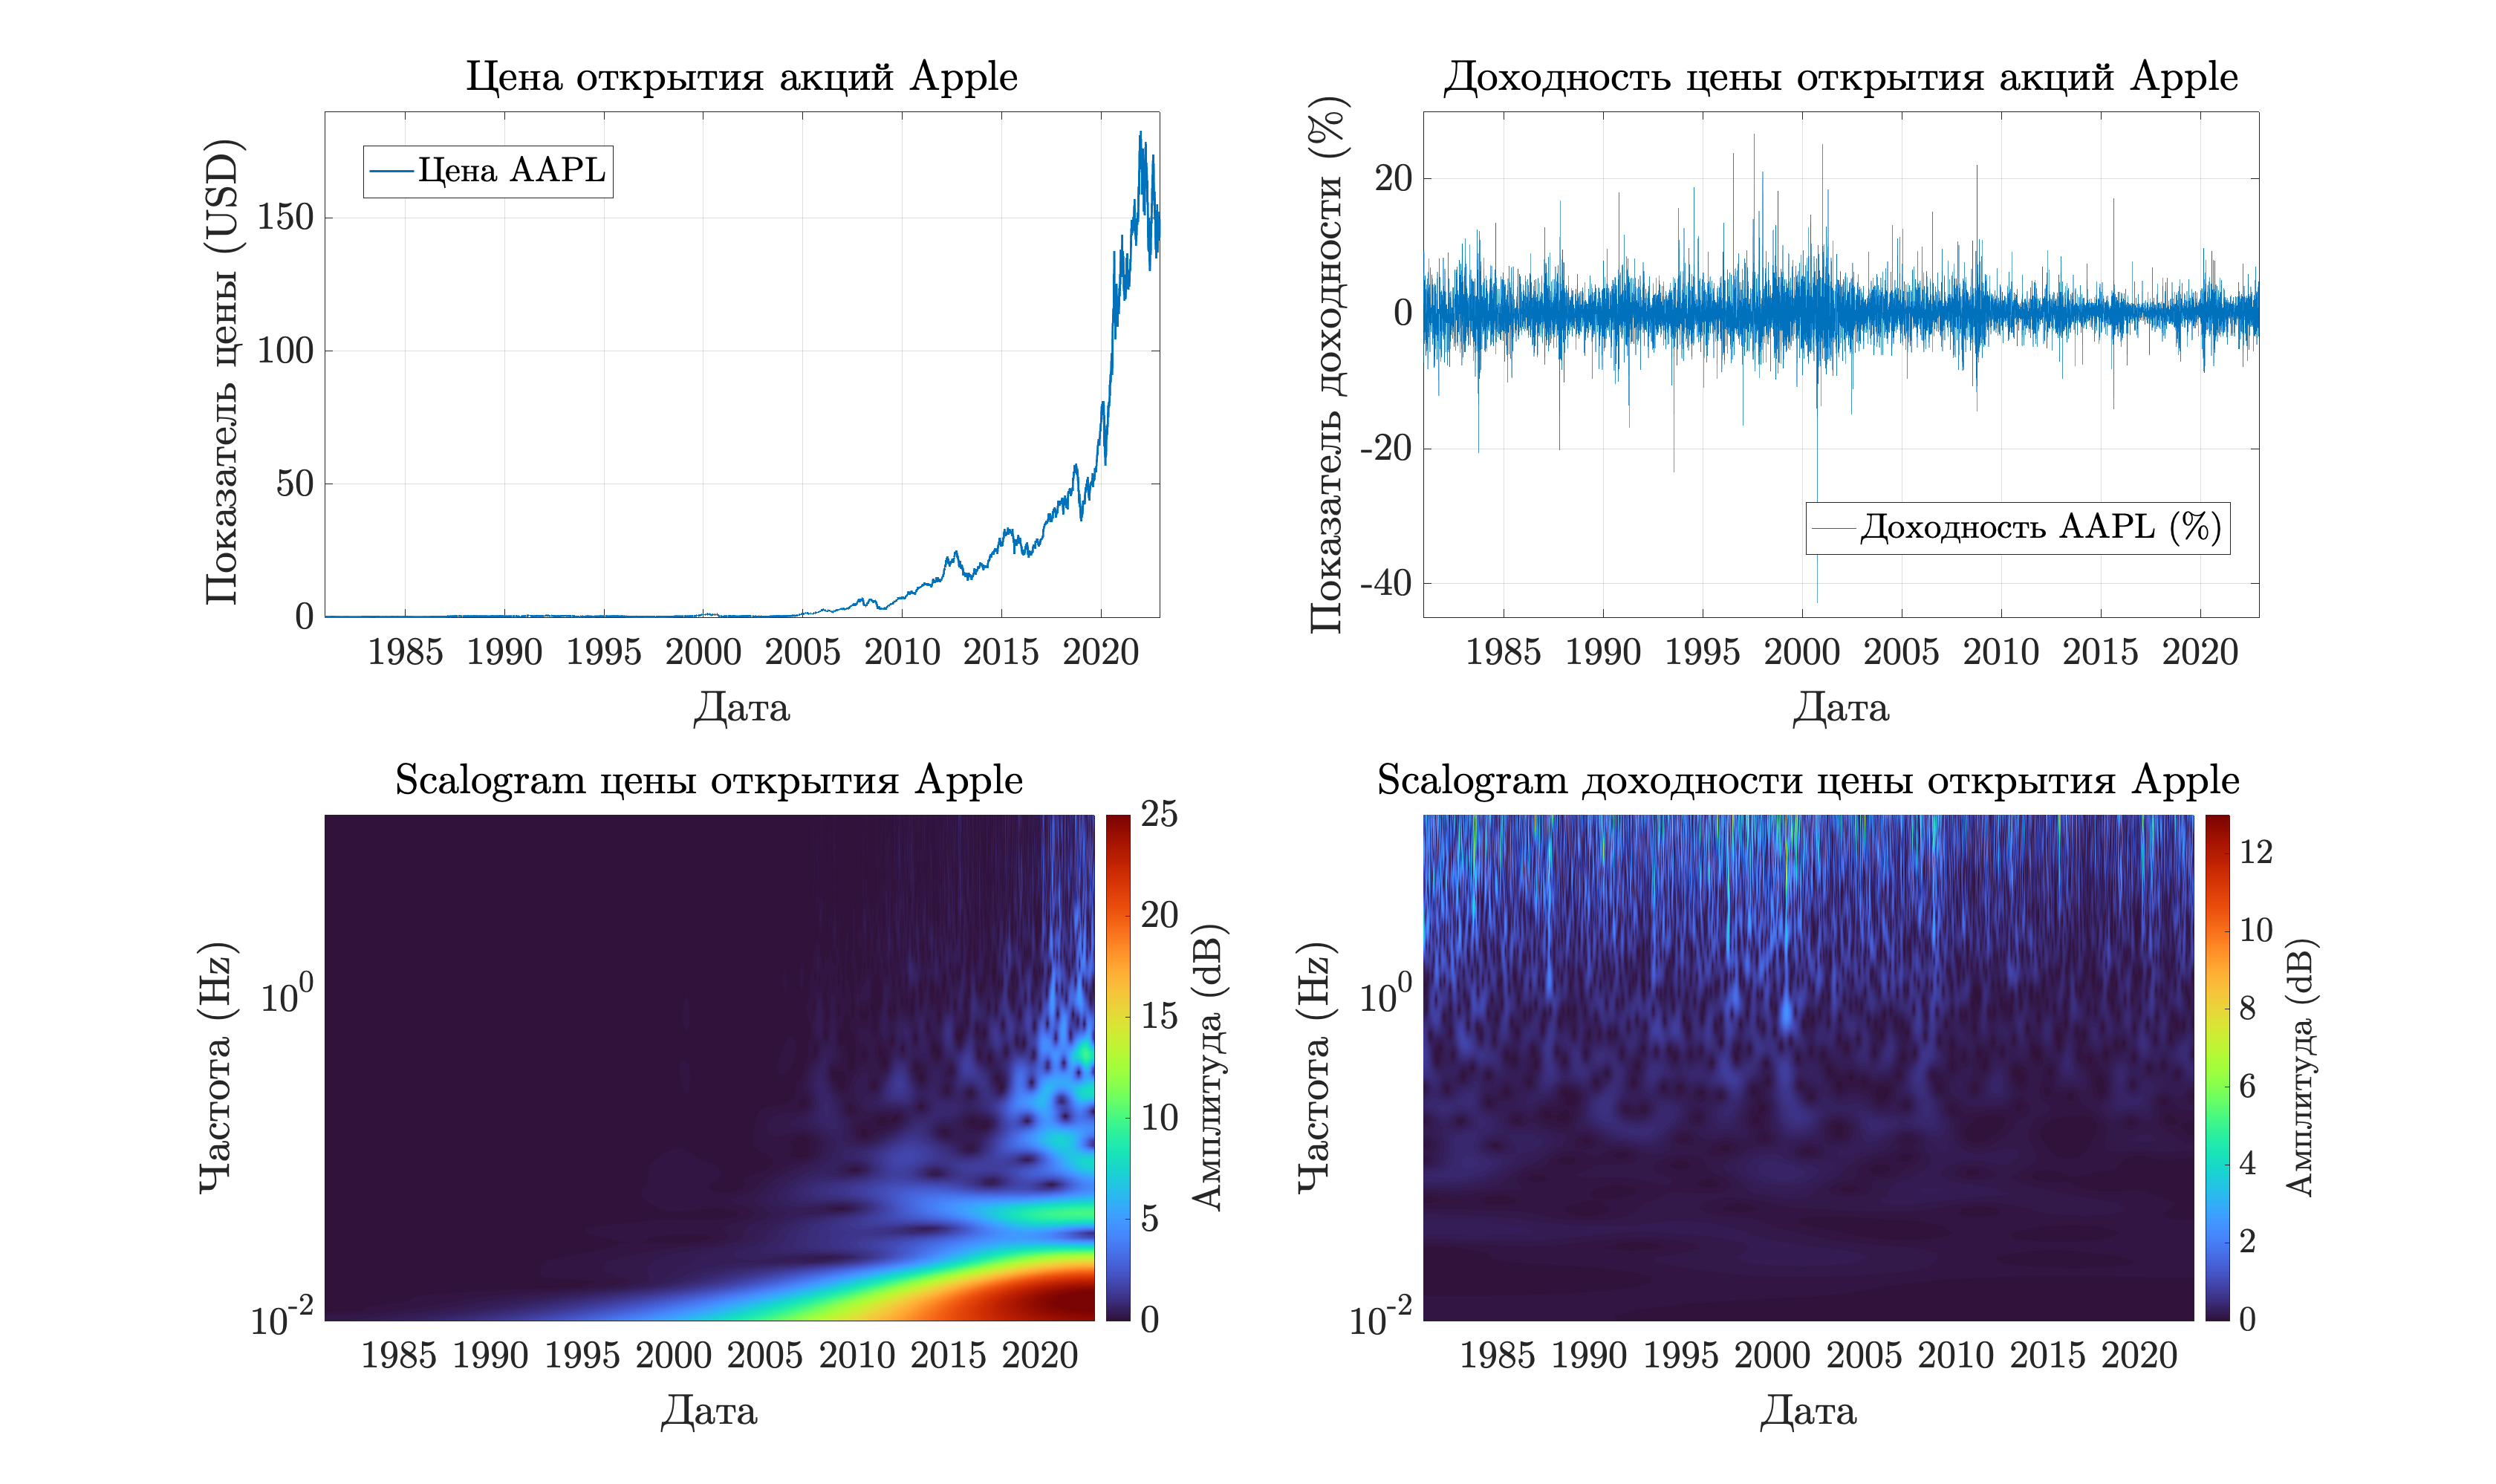
\includegraphics[width= 1.05\textwidth]{time frequency/scalogram_plots.png}
	\caption{График scalogram цены открытия и доходности Apple (IPO - 2022)}
	\label{fig::wavelet_example}
\end{figure}
Интересно, что теперь, по сравнению с анализом Фурье, четко выделено отсутствие какой-либо частотной информации для цен Apple, однако четко прослеживается очень большой ее объем в доходностях. Более того, наблюдая за негативными пиками в доходности, видим, что пики, падающие ниже $-20$ имеют четко выраженную лаговую структуру. В верхней части scalogram для доходностей существуют яркие пики, которые аккурат влекут за собой падение доходности, что аналогично предыдущему подтверждает наличие частотной информации в доходностях акций.

Однако конкретно данный алгоритм, как и преобразование Фурье, не получится использовать для прогнозирования, таким образом, их (алгоритмов) главная задача в настоящей работе - обеспечение очистки данных от шумовых компонент, обусловленных как погрешностью, так и временным лагом между наблюдениями - в случае Apple - это примерно $35$ часов.

Теперь приводим пример работы алгоритма очистки посредством применения WA (Wavelet Analysis). Рассматриваем все ту же функцию (\myref{link::illustr_func}).
\begin{figure}[H]
	\centering
	\begin{tikzpicture}
		\begin{axis}[
			grid = both,
			legend pos = north west,
			minor tick num = 1,
			major grid style = {lightgray},
			minor grid style = {lightgray!25},
			%title= {},
			width = \textwidth,
			height = 0.45 \textwidth,
			xmin=-5, xmax=5,
			ymin=-4, ymax=7.5,
			line width=0.3mm
			]
			
			\addplot[color = orange, line width = 0.035cm] table [
			x=x, 
			y=y_clean, 
			col sep=comma,
			mark={},
			] {./source/source_csv/Illustration data/wavelet/wavelet_example_denoising.csv};
			
			\addplot[opacity = 0.25, color = blue] table [
			x=x, 
			y=y_initial, 
			col sep=comma,
			mark={},
			] {./source/source_csv/Illustration data/wavelet/wavelet_example_denoising.csv};
			
			\addplot[domain = -5:5,
			samples = 300,
			color = teal,
			smooth,
			line width = 0.025cm,] {sin(deg(5 * x)) + 1 / 4 * (x^2)};
			
			\legend{$f(x)$ очищенный, $f(x)$ c шумом, $f(x)$ без шума};
		\end{axis}
	\end{tikzpicture}
	\caption{Очистка ряда от шума посредством преобразования Wavelet}
\end{figure}
Ошибка $\text{RMSE} = 0.7649$, что заметно больше, чем в случае применения метода MSSA, где ошибка $\text{RMSE} = 0.1744$ (\myref{link::mssa}). Таким образом, получаем, что для очистки от шума лучше использовать MSSA. Но в таком случае, появляется вопрос \textbf{Q}: Зачем весь этот метод тут, если, применяя его, не получается как прогнозировать (без специальных дополнительных предпосылок или теоретических выкладок, как, например, в статье \cite{schluter2010using}), так и лучше, чем MSSA очищать от шума (не строгое утверждение, а лишь основа на результате исследования настоящей работы)? \textbf{A}: Ответ присутствует в блоке (\myref{link::wavelet_nets}), где приводится описание применения Wavelet анализа к построению <<сетевых>> архитектур. Под <<сетевыми>> подразумеваются нейронные сети.

Таким образом, пока что вышеупомянутые методы Фурье и Wavelet преобразования остаются лишь прикладными к другим методам (это верно только для настоящей работы), так как напрямую для прогнозирования не применяются, однако это ничего не говорит об их качестве работы с анализируемыми данными. Далее переходим к описанию наиболее важной части текущего исследования, посвященной нейросетевому подходу к решению задачи прогнозирования показателей.